\documentclass[tikz,border=10pt]{standalone}
\usepackage[T1]{fontenc}
\usepackage{lmodern}
\usepackage{tikz}
\usetikzlibrary{arrows.meta,calc,decorations.pathreplacing,fit,matrix,positioning}

\definecolor{cornellred}{HTML}{B31B1B}
\definecolor{ink}{HTML}{202124}
\definecolor{muted}{HTML}{667085}
\definecolor{line}{HTML}{AEB8C6}
\definecolor{paper}{HTML}{FFFFFF}
\definecolor{soft}{HTML}{F5F7FA}
\definecolor{camera}{HTML}{E8F4FF}
\definecolor{memory}{HTML}{F0F7EC}
\definecolor{compute}{HTML}{FFF3E6}
\definecolor{display}{HTML}{F7ECF3}
\definecolor{verify}{HTML}{EFEAFE}

\tikzset{
  font=\sffamily,
  flow/.style={
    -{Latex[length=2.6mm,width=1.8mm]},
    draw=muted,
    line width=0.8pt,
    rounded corners=2pt
  },
  dataflow/.style={
    flow,
    draw=cornellred
  },
  block/.style={
    rectangle,
    rounded corners=3pt,
    draw=line,
    line width=0.8pt,
    fill=paper,
    align=center,
    minimum width=28mm,
    minimum height=10mm,
    inner xsep=4pt,
    inner ysep=4pt
  },
  smallblock/.style={
    block,
    minimum width=22mm,
    minimum height=8mm,
    font=\sffamily\scriptsize
  },
  title/.style={
    font=\sffamily\bfseries\large,
    text=ink
  },
  labeltext/.style={
    font=\sffamily\scriptsize,
    text=muted,
    align=center
  },
  camera_block/.style={block, fill=camera, draw=blue!45!black},
  memory_block/.style={block, fill=memory, draw=green!45!black},
  compute_block/.style={block, fill=compute, draw=orange!65!black},
  display_block/.style={block, fill=display, draw=purple!45!black},
  verify_block/.style={block, fill=verify, draw=violet!50!black},
  groupbox/.style={
    draw=line,
    rounded corners=5pt,
    line width=0.7pt,
    fill=soft,
    inner sep=7pt
  }
}

\usetikzlibrary{arrows.meta,positioning,fit,calc,decorations.markings}

\begin{document}
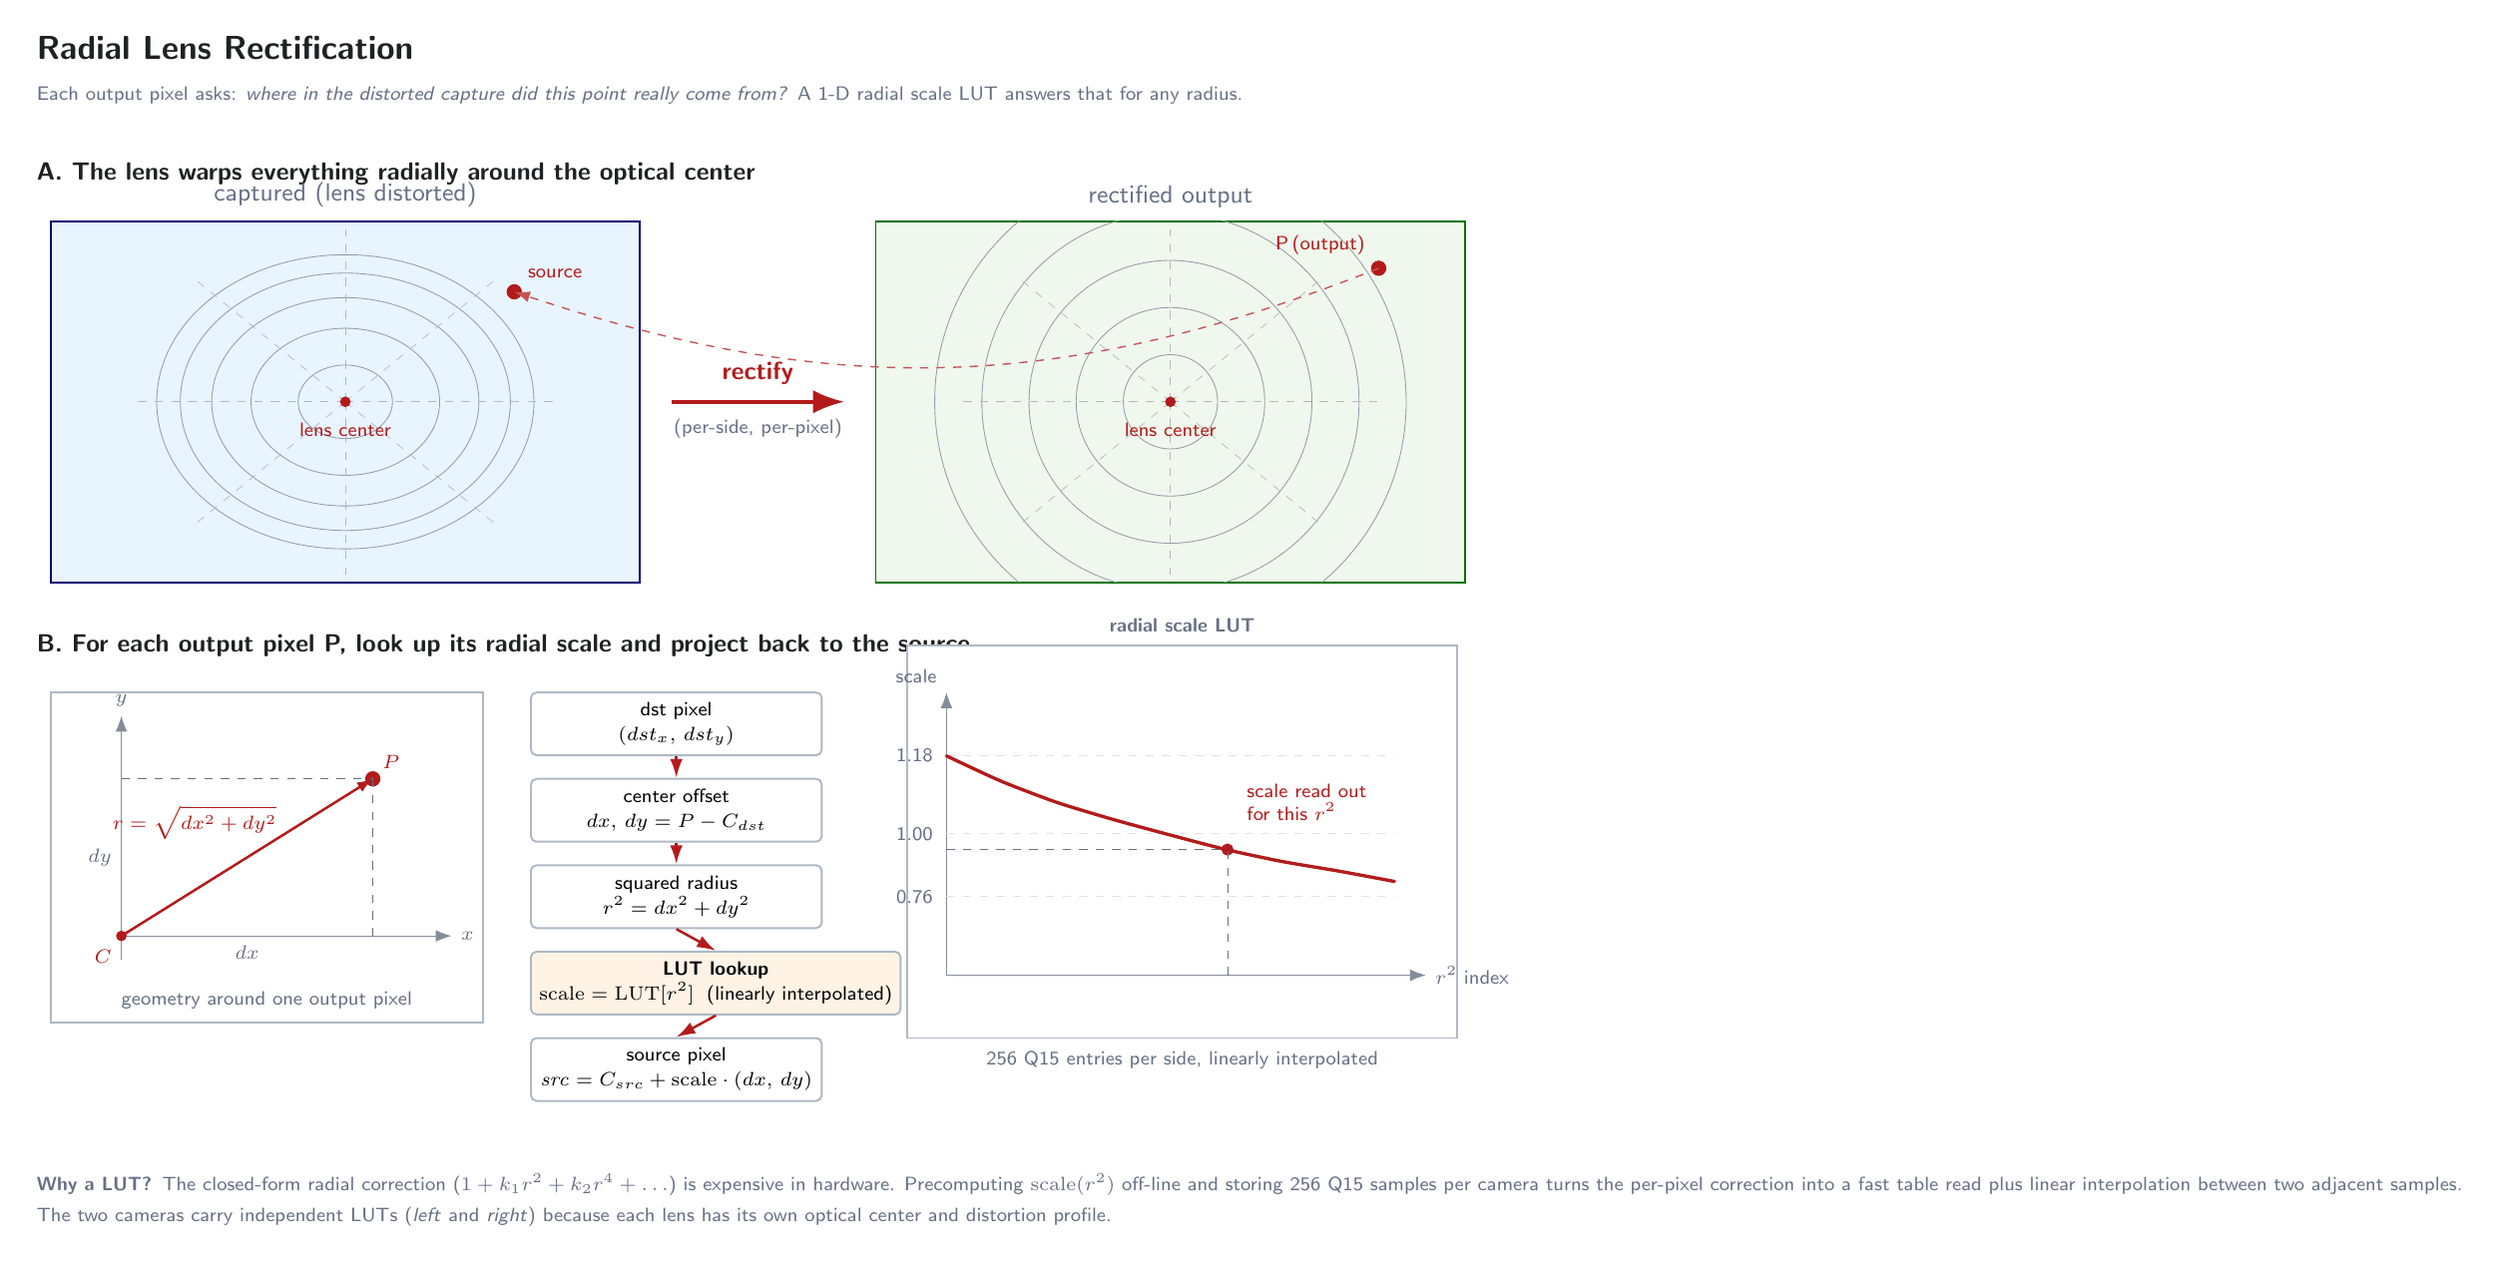
\begin{tikzpicture}[x=1mm,y=1mm,
  stage/.style={
    rectangle, rounded corners=2pt, draw=line, line width=0.7pt,
    fill=paper, align=center, font=\sffamily\scriptsize,
    inner xsep=3pt, inner ysep=3pt,
    minimum height=8mm
  },
  pipe/.style={
    -{Latex[length=2.4mm,width=1.6mm]},
    draw=cornellred,
    line width=0.9pt
  },
  axislbl/.style={font=\sffamily\scriptsize, text=muted}
]

  \node[title, anchor=west] at (0, 138) {Radial Lens Rectification};
  \node[labeltext, anchor=west] at (0, 132)
    {Each output pixel asks: \emph{where in the distorted capture did this point really come from?}
     A 1-D radial scale LUT answers that for any radius.};

  %====================================================================
  % SECTION A -- picture-level view: captured vs rectified
  %====================================================================
  \node[labeltext, anchor=west, text=ink, font=\sffamily\small\bfseries]
    at (0, 122) {A.\,\,The lens warps everything radially around the optical center};

  % --- Captured (distorted) -------------------------------------------
  \draw[fill=camera, draw=blue!45!black, line width=0.7pt]
    (3, 70) rectangle (78, 116);
  \node[labeltext, anchor=south, font=\sffamily\small] at (40.5, 116.5)
    {captured (lens distorted)};

  \begin{scope}
    \clip (3,70) rectangle (78,116);
    % bunched-up contours (denser near the edge)
    \foreach \r in {6, 12, 17, 21, 24} {
      \draw[muted!70, line width=0.3pt]
        (40.5, 93) ellipse [x radius=\r, y radius={\r*0.78}];
    }
    \foreach \a in {0, 45, 90, 135, 180, 225, 270, 315} {
      \draw[muted!50, line width=0.25pt, dashed]
        (40.5, 93) -- ({40.5+27*cos(\a)}, {93+22*sin(\a)});
    }
  \end{scope}

  \filldraw[cornellred] (40.5, 93) circle (0.6);
  \node[labeltext, anchor=north, text=cornellred, font=\sffamily\scriptsize]
    at (40.5, 91.5) {lens center};

  \coordinate (capP) at (62, 107);
  \filldraw[cornellred] (capP) circle (0.9);
  \node[labeltext, anchor=south west, text=cornellred,
        font=\sffamily\scriptsize] at (62.5, 107.5) {source};

  % --- Rectify arrow ---------------------------------------------------
  \draw[-{Latex[length=4mm,width=3mm]}, draw=cornellred, line width=1.4pt]
    (82, 93) -- (104, 93);
  \node[labeltext, anchor=south, text=cornellred, font=\sffamily\small\bfseries]
    at (93, 94) {rectify};
  \node[labeltext, anchor=north, text=muted, font=\sffamily\scriptsize]
    at (93, 92) {(per-side, per-pixel)};

  % --- Rectified (straight) -------------------------------------------
  \draw[fill=memory, draw=green!45!black, line width=0.7pt]
    (108, 70) rectangle (183, 116);
  \node[labeltext, anchor=south, font=\sffamily\small] at (145.5, 116.5)
    {rectified output};

  \begin{scope}
    \clip (108,70) rectangle (183,116);
    \foreach \r in {6, 12, 18, 24, 30} {
      \draw[muted!70, line width=0.3pt] (145.5, 93) circle (\r);
    }
    \foreach \a in {0, 45, 90, 135, 180, 225, 270, 315} {
      \draw[muted!50, line width=0.25pt, dashed]
        (145.5, 93) -- ({145.5+27*cos(\a)}, {93+22*sin(\a)});
    }
  \end{scope}

  \filldraw[cornellred] (145.5, 93) circle (0.6);
  \node[labeltext, anchor=north, text=cornellred, font=\sffamily\scriptsize]
    at (145.5, 91.5) {lens center};

  \coordinate (rectP) at (172, 110);
  \filldraw[cornellred] (rectP) circle (0.9);
  \node[labeltext, anchor=south east, text=cornellred,
        font=\sffamily\scriptsize] at (171.5, 110.5) {P\,(output)};

  % faint arc connecting the two example pixels to show the mapping
  \draw[dashed, draw=cornellred!75, line width=0.5pt,
        -{Latex[length=2mm,width=1.4mm]}]
    (rectP) to[bend left=20] (capP);

  %====================================================================
  % SECTION B -- per-pixel math
  %====================================================================
  \node[labeltext, anchor=west, text=ink, font=\sffamily\small\bfseries]
    at (0, 62) {B.\,\,For each output pixel P, look up its radial scale and project back to the source};

  % -- geometric inset on the left -------------------------------------
  \draw[fill=paper, draw=line, line width=0.6pt]
    (3, 14) rectangle (58, 56);
  \node[labeltext, anchor=south, font=\sffamily\scriptsize] at (30.5, 14.5)
    {geometry around one output pixel};

  \draw[muted!80, line width=0.35pt, -{Latex[length=2mm]}] (12, 25) -- (54, 25);
  \draw[muted!80, line width=0.35pt, -{Latex[length=2mm]}] (12, 22) -- (12, 53);
  \node[axislbl, anchor=west] at (54, 25) {$x$};
  \node[axislbl, anchor=south] at (12, 53) {$y$};

  \filldraw[cornellred] (12, 25) circle (0.6);
  \node[axislbl, anchor=north east, text=cornellred] at (12, 24.5) {$C$};

  \filldraw[cornellred] (44, 45) circle (0.9);
  \node[axislbl, anchor=south west, text=cornellred] at (44, 45) {$P$};

  \draw[muted, line width=0.4pt, dashed] (44, 25) -- (44, 45);
  \draw[muted, line width=0.4pt, dashed] (12, 45) -- (44, 45);
  \node[axislbl, anchor=north] at (28, 25) {$dx$};
  \node[axislbl, anchor=east] at (12, 35) {$dy$};

  \draw[cornellred, line width=0.9pt, -{Latex[length=2mm,width=1.4mm]}]
    (12, 25) -- (44, 45);
  \node[axislbl, anchor=south east, text=cornellred] at (33, 36)
    {$r=\sqrt{dx^2+dy^2}$};

  % -- pipeline on the right -------------------------------------------
  \node[stage, anchor=west, minimum width=37mm] (s1) at (64, 52)
    {dst pixel\\[1pt]$(dst_x,\,dst_y)$};
  \node[stage, anchor=west, minimum width=37mm] (s2) at (64, 41)
    {center offset\\[1pt]$dx,\,dy = P - C_{dst}$};
  \node[stage, anchor=west, minimum width=37mm] (s3) at (64, 30)
    {squared radius\\[1pt]$r^2 = dx^2 + dy^2$};
  \node[stage, anchor=west, minimum width=37mm, fill=compute] (s4) at (64, 19)
    {\textbf{LUT lookup}\\[1pt]$\mathrm{scale} = \mathrm{LUT}[r^2]$
     \;\scriptsize(linearly interpolated)};
  \node[stage, anchor=west, minimum width=37mm] (s5) at (64, 8)
    {source pixel\\[1pt]$\mathit{src} = C_{src} + \mathrm{scale}\cdot(dx,\,dy)$};

  \draw[pipe] (s1.south) -- (s2.north);
  \draw[pipe] (s2.south) -- (s3.north);
  \draw[pipe] (s3.south) -- (s4.north);
  \draw[pipe] (s4.south) -- (s5.north);

  % -- compact LUT curve on the right ----------------------------------
  \begin{scope}[shift={(112, 12)}]
    \draw[fill=paper, draw=line, line width=0.6pt] (0, 0) rectangle (70, 50);
    \node[labeltext, anchor=south, font=\sffamily\scriptsize\bfseries]
      at (35, 50.5) {radial scale LUT};
    \node[labeltext, anchor=north, font=\sffamily\scriptsize]
      at (35, -0.5) {256 Q15 entries per side, linearly interpolated};

    % axes
    \draw[muted!80, line width=0.35pt, -{Latex[length=2mm]}] (5, 8) -- (66, 8);
    \draw[muted!80, line width=0.35pt, -{Latex[length=2mm]}] (5, 8) -- (5, 44);
    \node[axislbl, anchor=west] at (66, 8) {$r^2$ index};
    \node[axislbl, anchor=south east] at (5, 44) {scale};

    % scale guides
    \node[axislbl, anchor=east] at (4.5, 36) {1.18};
    \node[axislbl, anchor=east] at (4.5, 26) {1.00};
    \node[axislbl, anchor=east] at (4.5, 18) {0.76};
    \draw[line!40, line width=0.3pt, dashed] (5, 36) -- (62, 36);
    \draw[line!40, line width=0.3pt, dashed] (5, 26) -- (62, 26);
    \draw[line!40, line width=0.3pt, dashed] (5, 18) -- (62, 18);

    % actual LUT curve -- coordinates derived from the real LUT values
    % (left side: 1.179, 1.094, 1.023, 0.966, 0.915, 0.866, 0.826, 0.794, 0.759
    %  at indices 0, 31, 63, 95, 127, 159, 191, 223, 255)
    \draw[cornellred, line width=1.2pt, line cap=round]
      plot[smooth, tension=0.4] coordinates {
        ( 5.00, 35.92)
        (11.93, 32.71)
        (19.08, 29.99)
        (26.24, 27.82)
        (33.39, 25.87)
        (40.54, 24.01)
        (47.70, 22.48)
        (54.85, 21.27)
        (62.00, 19.94)
      };

    % sample-lookup marker (near r^2 index 160)
    \filldraw[cornellred] (40.76, 24.0) circle (0.7);
    \draw[muted, line width=0.3pt, dashed] (40.76, 8) -- (40.76, 24.0);
    \draw[muted, line width=0.3pt, dashed] (5, 24.0) -- (40.76, 24.0);
    \node[axislbl, anchor=west, text=cornellred, align=left]
      at (42, 30) {scale read out\\for this $r^2$};
  \end{scope}

  %====================================================================
  % Footer
  %====================================================================
  \node[labeltext, anchor=north west, align=left] at (0, -4)
    {\textbf{Why a LUT?}\,
     The closed-form radial correction ($1 + k_1 r^2 + k_2 r^4 + \dots$) is expensive in hardware.
     Precomputing $\mathrm{scale}(r^2)$ off-line and storing 256 Q15 samples per camera turns the
     per-pixel correction into a fast table read plus linear interpolation between two adjacent
     samples.\\[3pt]
     The two cameras carry independent LUTs (\textit{left} and \textit{right}) because each lens
     has its own optical center and distortion profile.};

\end{tikzpicture}
\end{document}
